\subsection{Bilernes interaktion med andre mennesker}
I takt med at der kommer flere  selvkørende biler på vejene, er der kommet mere lys på de problemer som disse biler har når de har interaktioner med omgivelserne. En af de større udfordringer de har mødt, er selve trafikken og alt der hører med til denne. Bilens sensorer gør at den har en større årvågenhed end andre bilister, hvilket faktisk har vist sig at være et problem. Problemet er, at bilens opmærksomhed også sætter den i stor fare for at blive påkørt af en uopmærksom bilist som kommer kørende bagfra. Dette bekræfter Google selv i deres månedlige rapport fra august 2015\cite{GOOG_MONTHLY}. Et eksempel på dette skete på en travl vej i Mountain View Californien, hvor fodgængere kan trykke på en knap, for at få et lys på vejen til at skifte så de kan gå over. Her havde den selvkørende bil opdaget en person ude på dette fodgængerfelt, hvorefter testpersonen i bilen valgte  manuelt at bremse, for at sikre at de ikke ville ramme personen. Dog var bilen bag den selvkørende bil ikke lige så vågen, så den endte med at køre op bag i  den selvkørende bil. Det skal dog siges at trods den manuelle bremsning af testkøreren, så viste det sig senere at bilen selv ville være stoppet i tide. Dog ville den have kørt noget tættere på fodgængeren, hvilket kunne have virket skræmmende for fodgængeren\cite{GOOG_MONTHLY}. 

En anden udfordring de selvkørende biler har, er at som de er nu, kører ekstremt sikkert. I dette tilfælde skal ordet sikkert ikke tages på en god måde. Den selvkørende bil er bilen der virker som om den er lige lidt for langsom ude af lyskrydset, og som altid sikrer sig at den ikke overstiger fartgrænsen på nogen måde. Dette gør at den ellers travle trafik bliver sinket af de selvkørende biler som er på gaden. Denne form for kørsel ville i princippet ikke være et problem for bilen, men da der ikke er nogen mennesker der kører på helt samme måde, så skaber det som sagt nogle problemer. Et eksempel kunne være som vist på følgende figur.

\begin{figure}[h!]
    \centering
    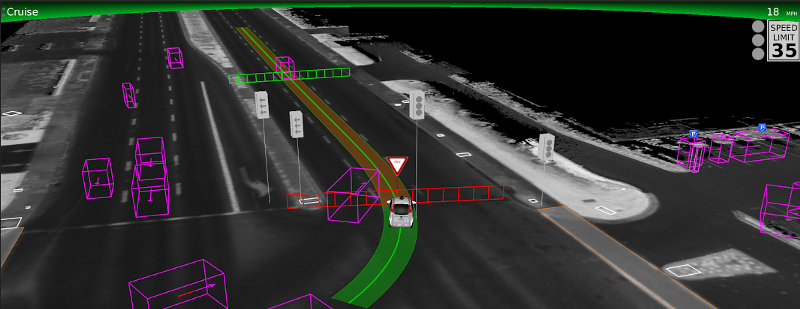
\includegraphics[width=0.8\textwidth]{images/google_vision.png}
    \caption{Bilens scan, der viser hvad der er i nærheden. Altså dens syn}
    \label{fig:car_vision}
\end{figure}

Figuren er taget af bilens syn på omverden under  en situation der virker godt som  et eksempel på dens kørsel. Her er de lyserøde kasser andre køretøjer, den grønne linje viser bilens planlagte rute, og midt i selve billedet er bilen selv. Men situationen her er, at bilen på den venstre side af den selvkørende bil svinger lidt bredt, da den har overset den selvkørende bil. Hvilket gør at den kommer ind i den selvkørende bils bane. Så i stedet for selv at tage et lidt bredere sving, så vælger den selvkørende bil at bremse ned. Dette tydeliggøres også på figuren, hvor der fremgår et rødt hegn foran bilen, hvilket  betyder at bilen bremser\cite{Backchannel}. En af de givne problemer mange byer er begyndt at møde, er at den store mængde mennesker der bor i disse byer, skal selvfølgelig have en form for transport. Dette er så biler, eller offentlig transport. Dette har gjort at selve byernes infrastruktur ikke har kunne følge med alle de mennesker der nu befinder sig på vejene, så den meget øgede trafik har gjort at kørsel i byerne er blevet meget aggresivt, for at komme hurtigere frem. Da tid brugt i trafikken kunne være brugt på en mere produktiv måde\cite{Michelin}. I sådanne et miljø ville den selvkørende bil både være en fordel og en ulempe. Det nemmeste ville selvfølgelig være hvis alle selv havde en selvkørende bil, da hele ruten ville kunne blive kalkuleret, så man ville kunne få en præcis tid for, hvor lang tid ruten ville tage, og man ville kunne lave noget andet samtidigt med at man kørte. Den store ulempe bilen vil have, er at hvis man som den eneste kører rundt i en selvkørende bil i disse områder vil det forstyre trafikken meget. Da de som nævnt tidligere kører meget sikkert, så gør den aggressive kørsel for de andre bilister, at den selvkørende bil vil kunne være en fare for sig selv, fordi den fx. ikke ville skynde sig over for et gult lys, men bilisten bag den tænkte at det var nået man godt kunne nå. Hvilket ville resultere i at den selvkørende bil ville blive kørt op i bag fra.

En anden situation hvor sådan en bil fejlede i at reagere blev beskrevet af en cyklist i Austin, Texas, hvor han nemlig mødte en sådanne selvkørende bil i et kryds, mens han var på cykel. Cyklisten lavede så det man kalder en track-stand, men han lagde sig ind bag bilen. En track-stand er en teknik man bruger til at holde sig på cyklen når man kører rigtigt langsomt, hvor man så også bevæger styret på cyklen frem og tilbage for at holde balancen. Den selvkørende bil misforstod så denne track-stand for en cyklist der kom kørende bag den og stoppede. Så da bilen kunne se at cyklisten holdt stille kørte den så igen, hvorefter den så stoppede igen fordi cyklisten bevægede styret fra den ene side til den anden. Dette gjorde at bilen stadig ikke var nået ud til midten af krydset efter hele 2 minutters kørsel\cite{VOX}. Det lyder måske ikke af meget, men det er sådanne problemer man er nød til at sikre ikke sker efter bilen er udgivet til private personer, da begge hændelser ville have kunne føre til større ulykker, yderligere forsinkelser af trafikken eller fører til personskader. 